\subsubsection{Conexionado del sistema}\label{subsec:conexionado}

El sistema funciona principalmente gracias al panel solar. Este se encarga de alimentar el circuito y cargar las 3 baterías (\texttt{BACKUP}, \texttt{BAT1} y \texttt{BAT2}). Para ello, ofrece una tensión de entorno a los $24 V$. Si se detecta que la tensión obtenida del panel es inferior a cierto umbral definido en el código, el circuito pasa a alimentarse con la batería de backup.

El panel solar se conecta a un \texttt{INA226} para poder medir su tensión y corriente, y después se conecta a los dos relés. El relé 1 se encarga de conectar el panel solar al cargador de la batería de backup para poder cargarla, mientras que el relé 2 se encarga de elegir la alimentación del circuito (Solar o backup).

Entre el relé 1 y el cargador de la batería de backup hay un diodo. Este diodo evita la corriente inversa del cargador. Cabe destacar que este diodo no se ha colocado en la batería dado que evitaría corriente saliente de la batería, por lo que no permitiría utilizar la batería de backup como alimentación.

El cargador de la batería de backup se conecta a la batería de backup y a los \texttt{INA226} para poder medir la tensión y corriente de la batería de backup. La batería de backup, para que pueda alimentar al circuito, se conecta a un regulador conmutado elevador, para convertir los $12 V$ que entrega a $24 V$. Este regulador se conecta al relé 2 para poder alimentar el circuito.

Del relé 2 sale la alimentación del circuito, solar o backup según como esté conmutado el relé. Esta alimentación se conecta a los cargadores de las baterías 1 y 2 y a un regulador conmutado reductor. Los cargadores de las baterías 1 y 2 se conectan a las baterías 1 y 2 respectivamente con los \texttt{INA226} para poder medir la tensión y corriente de las baterías.

Entre la salida del relé 2 y cada cargador de batería hay un diodo. Este diodo, al igual que el de la de backup, evita la corriente inversa por el cargador. Cabe destacar que no se conecta entre el cargador y el \texttt{INA226}, ya que a la tensión para cargar la batería se le restaría la caída de tensión en el diodo, por lo que no se cargaría correctamente y para los $24 V$ que entrega la alimentación sí se puede permitir la caída de tensión del diodo. Del mismo modo, tampoco se puede colocar entre el \texttt{INA226} y la batería dado que no permitiría medir correctamente la tensión y corriente de carga de la batería, además de que seguiría existiendo el problema con la caída de tensión.

El regulador conmutado reductor se encarga de reducir los $24 V$ de su entrada a $7 V$ en la entrada del \texttt{LDO}. La salida del \texttt{LDO} se conecta a los \texttt{INA226} y al \texttt{ESP8266} para alimentarlos a $5 V$.

Para medir la tensión y corriente en el panel solar, la batería de backup y las baterías principales, se utilizan los \texttt{INA226}. Estos sensores se conectan al \texttt{ESP8266} por \texttt{I2C}, que se encarga de procesar la información y enviarla por \texttt{MQTT} al servidor, además de guardarla en un \texttt{log}.

El \texttt{ESP8266} se encarga no solo de la toma y gestión de las medidas sino que también del control de la conmutación de los relés para los cambios de estado del sistema [\autoref{subsubsec:estados}] y la protección del circuito. Por ello, dos de sus pines están conectados a la entrada \texttt{SW} de cada relé.

En la \autoref{fig:hardware/conexiones} se muestra el diagrama de conexiones del sistema:

\begin{figure}[H]
    \centering
    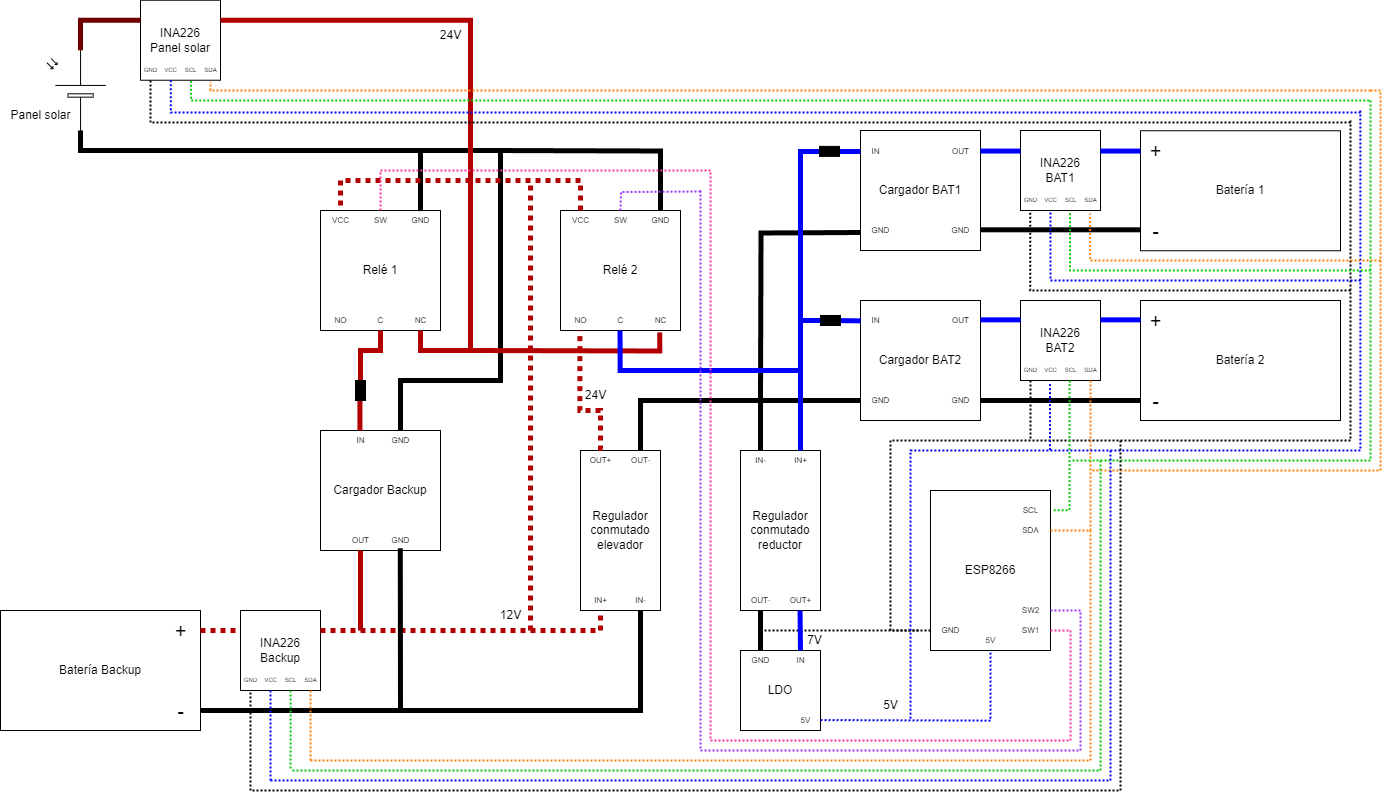
\includegraphics[width=0.95\textwidth]{images/2-hardware/Conexiones.png}
    \caption{Conexiones del sistema}
    \label{fig:hardware/conexiones}
\end{figure}
